\chapter{A brief history of molecules}\label{ch:history}

\vspace{-1.5 em}
\begin{addmargin}[-0.5cm]{0cm}
  \minitoc
\end{addmargin}
\hrule
\vspace{1.5 em}

What is Coulomb explosion imaging? A technical definition could be given, however, it is simply a decades-old technique in a long line of techniques stretching back centuries, all meant to answer a question posed by the ancient Greeks and Indians---what are the building blocks of the universe, and how do they behave?

It is easy to get stuck in the ivory tower and get lost within the trees of science, losing sight of the big picture of where your research leads.

\section{Atomism: an ancient question}

\section{Seeing molecules and saving lives}

\section{Molecular movies}
Molecular movies are of course not only of interest in physics and chemistry as a means of probing fundamental processes, but also in the biological sciences where molecular structure play a crucial role in determining the function of biomolecules such as proteins. However, the molecules of interest there are much too large to be studied by any of the previous techniques. Thus molecular movies in the biological sciences tend to be annotated computer simulations amalgamated from multiple studies. That said, they are very impressive pieces of work.

A particularly impressive movie by \citet{Cheung12} showcases the process of RNA polymerase transcription and goes on for over six minutes.

% FOCUS ON THE HISTORY OF CEI IN DETERMINING GEOMETRIES
\section{Coulomb explosion imaging}
The original CEI experiment is usually traced back to \citet{Vager89} in which the Coulomb explosion is initiated by passing a molecular beam through a thin foil. This may be because it was the first work suggesting that full molecular structures may be recovered by measuring the velocity (or momentum) vectors of the atomic fragments, and even reported on a non-classical molecular structure. However, previous works utilizing CEI do exist, even some significant works that report on molecular structures \citep{Kanter79}.

Ultrashort laser pulses\footnotemark as a means of inducing Coulomb explosions made their entrance in the 1980's where they were utilized to infer molecular dynamics using covariance mapping \citep{Frasinski89}. Highly charged ion impact is another method of inducing a Coulomb explosion, and was first done in the 1990's in parallel with the development of more sophisticated coincidence mapping techniques. Since then, the laser has emerged as the more popular tool and has further developed the coincidence mapping technique. There do exist other methods of inducing Coulomb explosions, for example, single photons from a synchrotron source utilizing the Auger effect, x-ray pulses from a free-electron laser source, or electron collision.

\footnotetext{In 1987, ultrashort would be referring to \SI{0.6}{\pico\s} laser pulses \citep{Frasinski87}.}

In this section we will trace the history of CEI back to the 1970's where it started with foil-induced fragmentation. We will then follow it's development to the present day where ultrashort laser pulses are the most popular means of performing CEI. Throughout we will focus solely on the achievements of CEI in determining molecular structures, and in creating molecular movies using these recovered structures.\footnotemark

\footnotetext{Much of the molecular dynamics are inferred in CEI from studying the distribution of the fragment momentum vectors (\eg through the use of Newton and Dalitz plots) and the distribution of kinetic energy carried away by each fragment. We will be focusing on the original aim of CEI, that is, to measure molecular structures.}

Interestingly, the first-ever mention of the term ``Coulomb explosion'' in the published literature comes from an unrelated study of the fine structure of singly ionized helium by \citet{Novick55}. They measured the energy difference of the $2 \, ^2 S_{1/2}$ and $2 \, ^2 P_{1/2}$ states of ionized helium as a sensitive test of quantum electrodynamics. Coulomb explosion (or space charge explosion) was the dominant ion removal mechanism which they accounted for in modeling the quenching rate\footnotemark of metastable $2 \, ^2 S_{1/2}$ ions by radio frequency radiation to describe the observed resonance lineshapes (spending two appendices on it).

\footnotetext{The term was more popular in decades past but simply means the extinction rate or loss rate of metastable ions.}

\subsection{Foil-forged images}
CEI was first performed by passing a molecular beam containing the molecule of interest through a thin atomic film. Figure \ref{fig:foilExperiment} shows a schematic of such an experiment. While in the solid film, the probability for Coulomb scattering of the individual atomic nuclei is small due to their small size and consequently small interaction cross-section. However, the electrons will be scattered to very wide angles due to their interaction with the many electron clouds in the film. This process rapidly ionizes the molecule, typically within the first few atomic layers or the first femtosecond. The now highly ionized molecule exits the foil and rapidly dissociates into its consituent atomic fragments which repel eachother under their mutual Coulomb repulsion in what is termed a ``Coulomb explosion''.

\begin{figure}[H]
  \centering
  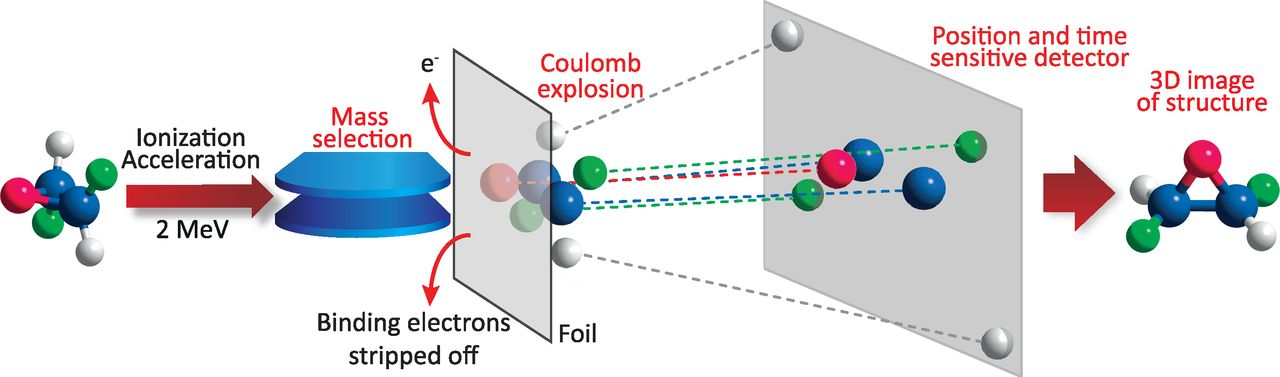
\includegraphics[width=\textwidth]{gfx/FoilExperiment}
  \caption[Schematic of a foil-induced Coulomb explosion imaging experiment.]
  {Schematic of a foil-induced Coulomb explosion imaging experiment. This specific experiment set out to measure the absolute configuration of atoms in a chiral molecule in the gas phase, which remains challenging. Early foil-induced CEI experiments can be described by this schematic except for the fact that they did not employ a mass selector and used a more primitive but still position-sensitive detector. The atomic fragment trajectories (dashed lines) assume that no rearrangement of the atoms occurs and that the system evolves under a Coulomb potential. From \citet{Herwig13}. Reprinted with permission from AAAS.}
  \label{fig:foilExperiment}
\end{figure}

The premise behind foil-induced CEI is that during this explosion, the atoms simply repel each other and do not rearrange, thus preserving the angles between them from the time they exit the foil to the time they are detected at a position and time-sensitive detector. As the potential energy of each pair of fragments $i,j$ is coverted to kinetic energy according to
$$ \frac{4q_i q_j}{|\mathbf{r}_i - \mathbf{r}_j|} = \frac{\mu|\mathbf{V}_i - \mathbf{V}_j|^2}{2} $$
it suggests that measurement of the asymptotic vector velocities completely defines the initial geometry of the molecule \citep{Vager89}. Here $q_i$, $\mathbf{r}_i$, and $\mathbf{V}_i$ are the charge, position vector, and velocity vector of the atomic fragment $i$ while $\mu$ is the reduced mass of the two-body system of fragments $i,j$.

Of course, there are some assumptions that must hold for a complete and accurate recovery of the initial geometry. It is important to understand when CEI works.

The earliest example of a molecular geometry recovered using CEI is reported by \citet{Gaillard78}. They used the foil-induced Coulomb explosion to image the structure of the \ch{H3+} molecular ion, showing that it is mainly exhibits an equalaterial triangular shape in three completely different experiments.\footnotemark ~Figure \ref{fig:hydrogenTrimer} gives a few examples of the geometries they recovered.

\footnotetext{It is interesting to note that the experiment was repeated by separate teams at the Argonne National Laboratory, the Université Claude Bernard Lyon 1, and the Weizmann Institute of Science, then reported on in one manuscript.}

\begin{figure}
  \centering
  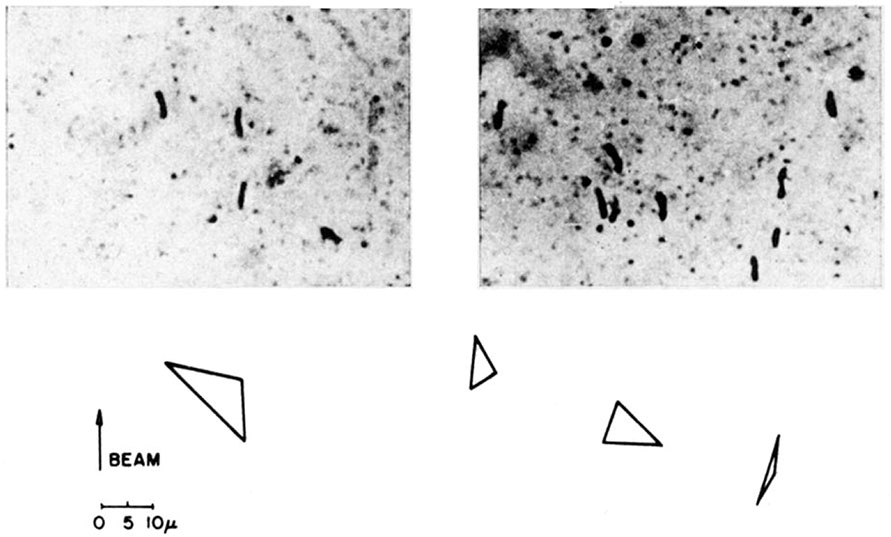
\includegraphics[width=\textwidth]{gfx/HydrogenTrimerReconstruction}
  \caption[Reconstructions of exploded \ch{H3+} following foil-induced dissociation.]
  {Reconstructions of exploded \ch{H3+} following foil-induced dissociation. On the top row are a couple of good photographs of exploded \ch{H3+} recorded on photographic emulsion at a tilt angle of $30\degree$. The bottom row shows a few reconstructions (normally projected) made by inspection from the photographs. The authors analyzed 350 such photographs and concluded that \ch{H3+} mainly exhibits an equalateral triangle geometry. From \citet{Gaillard78}. Reprinted with permission from APS.}
  \label{fig:hydrogenTrimer}
\end{figure}

CEI was first performed by \citet{Vager89} whereby the Coulomb explosion was initiated by passing a molecular beam through a thin ($\sim$\SI{30}{\angstrom}) aluminum film at high velocities ($\sim$$0.02c$). Their work was motivated by the opportunity of imaging non-classical molecular structures that more popular methods were incapble of seeing. They were also the first to suggest that measuring the velocity (or momentum) vectors of each fragment would be provide all the information required to describe the molecule's structure. Specifically for methane (\ch{CH4}), they state that the \ch{H-C-H} bond angles are preserved and that the potential energy of each \ch{C-H} pair is coverted to kinetic energy according to
\begin{equation}
\frac{4e^2}{|\mathbf{r}_C - \mathbf{r}_n|} = \frac{\mu|\mathbf{V}_C - \mathbf{V}_n|^2}{2}
\end{equation}
such that measurements of the asymptotic vector velocities completely defines the initial geometry of the molecule.

However, they do not perform any geometry reconstruction and report their fragment ion densities in a coordinate system defined by the asymptotic velocity of each particle, and claim that it is a direct measurement of the square of the multidimensional wave function of a many-body system.

%\begin{SCfigure}
%  \centering
%  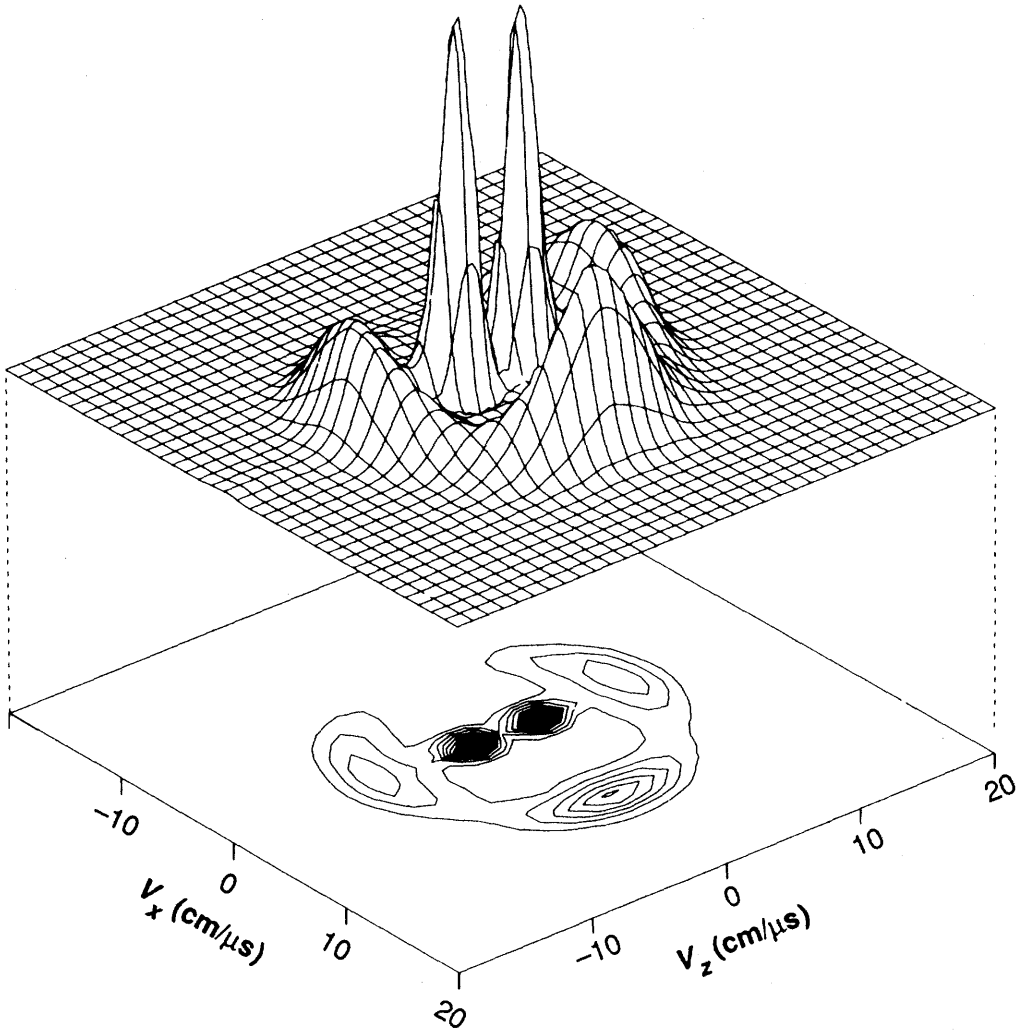
\includegraphics[width=0.5\textwidth]{gfx/VagerPseudoGeometry}
%  \caption[Reconstruction of \ch{C2H3+} following foil-induced dissociation.]
%  {Reconstruction of \ch{C2H3+} following foil-induced dissociation. From \citet{Vager89}. Reprinted with permission from AAAS.}
%\end{SCfigure}

%\begin{figure}
%  \centering
%  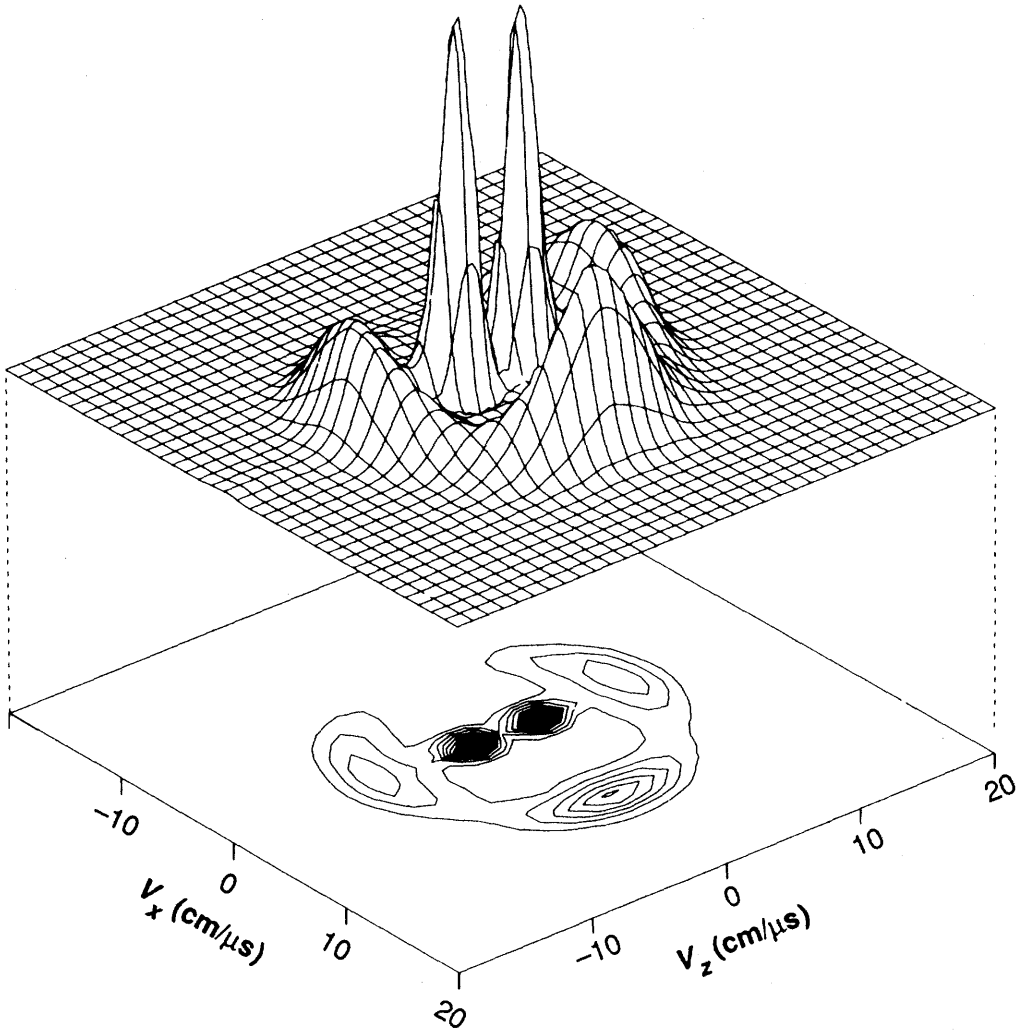
\includegraphics[width=\textwidth]{gfx/VagerPseudoGeometry}
%  \caption[Reconstruction of \ch{C2H3+} following foil-induced dissociation.]
%  {Reconstruction of \ch{C2H3+} following foil-induced dissociation. From \citet{Vager89}. Reprinted with permission from AAAS.}
%\end{figure}

One drawback of initiating Coulomb explosions using a thin foil is that a molecular beam must be prepared.

\subsection{Fragmentation by highly charged ion impact}

\subsection{Laser-induced dissociation}
\index{Classical imaging formula}
\index{Coulomb explosion imaging!Classical imaging formula}
Before taking a tour of the molecular geometries recovered using laser-induced CEI, it is worth mentioning that \citet{Nagaya04} have attempted to arrive at an analytical solution for calculating molecular geometries from measured momentum vectors. They were able to derive a ``classical imaging formula''
\begin{equation}
|\Psi_\mathrm{image}(R_I)|^2 = S(p) \frac{1}{P_\mathrm{ion}(R_I)} \sqrt{\frac{\mu q_A q_B}{8\pi\epsilon_0 R_I^3}} , \quad R_I = \frac{\mu q_A q_B}{2\pi\epsilon_0 p^2}
\end{equation}
where
\begin{equation}
S(p) = |c(p)|^2 = \left| \int \Phi_C^*(p,r) T_\mathrm{ion}(r) \Psi(r) \; dr  \right|^2
\end{equation}
for the position wavefunction of a molecule in terms of its momentum distribution $S(p)$. They are able to derive a similar formula for the Coulomb explosion of a symmetric linear triatomic molecule, but the more general case of the asymmetric linear triatomic molecule proves much more formidable.\footnotemark ~They proceed to compare their ``classical'' reconstructions for the vibrational wavefunction of a helium trimer system to the predictions of the quantum theory, noting small discrepencies.

\footnotetext{The bulk of their article focuses on the Coulomb explosion of asymmetric linear triatmoic molecules and derives a two-dimensional classical imaging formula in terms of hyperspherical coordinates. An extension to three dimensions for bent triatomic molecules is promised but could not be found in the published literature. While a highly commendable effort, their unsaid conclusion seems to be that this is an intractable problem as their research group seems to have gone silent on this problem and the only citations to this work are in the context of the difficulty of the problem.}

\citet{Legare05structure,Legare05dynamics} were the first to use ultrashort laser pulses and CEI to report on molecular structures and dynamics. To obtain the structures, they assume the explosion system evolves under a purely Coulombic potential and use optimization methods\footnotemark~ to make guesses at the structure that most accurately reproduces the observed data consistent with minimizing a least-squares objective function.

\footnotetext{Dissapointingly, they trivialize the solution to a couple of sentences and fail to report the optimization methods employed, sidestepping the nuances of the reconstruction process that we will discuss in chapters \ref{ch:lookupTable}--\ref{ch:bayesian}. The nuances include the existence, in some cases, of multiple molecular structures producing the same momentum vector distribution and the high sensitivity of the reconstructed initial geometry to uncertainties in the momentum vectors leading to very uncertain geometries in some cases. They also apply convex optimization methods to a problem that is not convex.}

Using \SI{8}{\fs} laser pulses they report on the structure of \ch{D2O} and \ch{SO2} \citep{Legare05structure}. They also claim to have imaged vibrating \ch{D2+} and dissociating \ch{SO2^{2+}} and \ch{SO2^{3}} however they provide no more than a couple of dissociation frames and infer the transient \ch{D2+} bond length from kinetic energy release ratios as a function of pump-probe time delay \citep{Legare05dynamics}.

\citet{Gagnon08} reported the reconstruction of dichloromethane (\ch{CH2Cl2}) using a home-made \footnotemark stochastic-based simulated annealing algorithm that globally optimizes the molecular spatial configuration. They discuss uncertainties but are only able to obtain the structure in five cases.

\footnotetext{There is nothing wrong with writing your own code here but nonconvex optimization algorithms are tricky to get right and the reliance should be on professional code.}

\index{Lookup table}
The best effort so far has probably been the one by \citet{Kunitski15} in which they use a lookup table approach to image the elusive Efimov state of the helium trimer.